\documentclass[notitlepage, twocolumn, 10pt]{article}

\usepackage[left=0.6in, right=0.6in, top=0.8in, bottom=0.8in]{geometry}
\usepackage{titling}
\usepackage[compact]{titlesec}
\usepackage{lipsum}
\usepackage{graphicx}
\usepackage[labelfont=bf, labelsep=space, font=small]{caption}
\usepackage[labelformat=simple]{subcaption}
\usepackage[noabbrev]{cleveref}
\usepackage{mwe}
\usepackage{sansmathfonts}
\usepackage{amsmath}
\usepackage{float}
\usepackage{fancyhdr}
\usepackage{multicol}
\usepackage{booktabs}
\usepackage{stfloats}
\usepackage[colorlinks=true,linkcolor=black,anchorcolor=black,citecolor=black,menucolor=black,runcolor=black,urlcolor=black,bookmarks=true]{hyperref}
\usepackage[flushleft]{threeparttable}
\usepackage[noblocks, affil-it]{authblk}
\usepackage{enumerate}
\usepackage[english]{babel}
\usepackage[numbers, super, sort&compress]{natbib}
\usepackage[group-separator={,}]{siunitx}
\usepackage{xcolor}
\usepackage{colortbl}
\usepackage[T1]{fontenc}
\usepackage{lmodern}

\pagestyle{fancy}
\fancyhf{}
\fancyhead[LE,RO]{}
\fancyhead[RE,LO]{}
\fancyfoot[CE,CO]{}
\fancyfoot[LE,RO]{\thepage}

\renewcommand{\headrulewidth}{0.5pt}
% \renewcommand{\footrulewidth}{0.5pt}

% set fonts
\renewcommand{\familydefault}{\sfdefault}
\captionsetup[figure]{font={sf, footnotesize}}

\titleformat*{\section}{\large\bfseries}
\titleformat{\subsection}[runin]{\bfseries}{}{}{}[.\:]

\titlespacing*{\section}{0pt}{\baselineskip}{1pt}
\titlespacing*{\subsection}{0pt}{0.5\baselineskip}{1pt}

\newcommand\invisiblesection[1]{%
  \refstepcounter{section}%
  \addcontentsline{toc}{section}{\protect\numberline{\thesection}#1}%
  \sectionmark{#1}\phantom{}}

\newcommand{\specialcell}[2][c]{%
  \begin{tabular}[t]{@{}c@{}}#2\end{tabular}}

\DeclareCaptionFormat{myformat}{#1#2#3}
\DeclareCaptionLabelFormat{bold}{\textbf{#2}}
\captionsetup[figure]{format=myformat, subrefformat=bold, name={Fig.}}
\captionsetup[subfigure]{format=default}
\captionsetup{justification=raggedright,singlelinecheck=false}

\definecolor{khaki}{rgb}{0.76, 0.69, 0.57}
\definecolor{lightgray}{rgb}{0.66, 0.6, 0.53}
\captionsetup[table]{box=colorbox,boxcolor=lightgray!20}

\makeatletter 
\renewcommand\@biblabel[1]{#1.} 
\makeatother
\def\bibfont{\footnotesize}
\setlength{\bibsep}{0pt}

\pretitle{\huge\normalfont\bfseries}
\posttitle{\par\vskip 0.5em}
\preauthor{\bfseries}
\postauthor{}
\predate{\par\large\centering}
\postdate{\par}

\renewcommand*{\Affilfont}{\normalsize\normalfont}
\renewcommand*{\Authfont}{\bfseries}    % make author names boldface 
\makeatletter
\renewcommand\AB@affilsepx{. \protect\Affilfont}
\makeatother

\title{Evaluating small-variant genotyping errors in polyploids}

\author[1,*]{Daniel P Cooke}
\author[2]{David C Wedge}
\author[3,1]{Gerton Lunter}
\affil[1]{\footnotesize MRC Weatherall Institute of Molecular Medicine, University of Oxford, Oxford, UK}
\affil[2]{\footnotesize Manchester Cancer Research Centre, University of Manchester, Manchester, UK}
\affil[3]{\footnotesize Department of Epidemiology, University Medical Centre Groningen, Groningen, The Netherlands}
\affil[*]{\footnotesize Correspondence should be addressed to D.P.C (dcooke@well.ox.ac.uk)}

\date{}

\begin{document}

\renewcommand{\abstractname}{\vspace{-\baselineskip}} % Remove Abstract header

\thispagestyle{empty}

\twocolumn[
  \begin{@twocolumnfalse}
  \maketitle
\noindent\textbf{%
The accuracy of polyploid genotyping from sequencing impacts several active research areas, notably plant breeding. However, compared with the situation for diploids, where comprehensive ground truth sets and robust benchmarking tools are standard, polyploids have been neglected; there are no benchmarks considering genotype errors for small variants using real data. Genotyping accuracy from sequencing in polyploids is therefore essentially unknown. We previously introduced a variant calling method - Octopus - that  accurately calls germline variants in diploids and somatic mutations in tumors. Here, we evaluate Octopus and other popular tools on whole-genome polyploid Illumina and PacBio HiFi data by \textit{in silico} mixing of diploid Genome In a Bottle samples. We find that polyploid genotyping errors are abundant for typical sequencing depths, but Octopus makes less than half the errors of other methods. We show our results give a credible upper-bound on performance in real polyploids by evaluating autotriploid banana and autotetraploid potato datasets.
%
}
\vspace{\baselineskip}
\end{@twocolumnfalse}
]

\invisiblesection{Motivation}
\vspace{-\baselineskip}

\noindent Polyploidy is common in many plant species, including important agricultural crops such as wheat, potato, oat, coffee, rapeseed, cotton, banana, and sugar cane \cite{RN658}. In mammals, polyploidization regularly occurs during tumorigenesis, but has also been shown to be a normal part of development in some mouse and humans tissues \cite{RN657}. Molecular markers have been widely used for decades in artificial polyploid crop breeding that aim to improve resilience to climate change and disease. More recently, sequencing of polyploids for genotyping and genome assembly has been used, and several high-quality reference genomes have been assembled \cite{RN668, RN671, RN659, RN664, RN660}. Despite these advances, methods for genotyping polyploids from sequencing data has received little scrutiny in comparison to those for diploids \cite{RN651, RN605, RN675}.

Variant calling and genotyping in polyploids is more difficult than in diploids primarily because the number of possible genotypes at a given loci is combinatorial in the ploidy and number of alleles, but sequencing reads are only informative of distinct alleles. It therefore becomes more difficult to determine the copy number of a particular allele for a fixed read depth as the ploidy increases. Moreover, since variant allele observations in the reads are expected to occur proportionally to the copy number divided by the sample ploidy, the ability to distinguish sequencing error from true variation diminishes as copy-number decreases and ploidy increases. Haplotype-based methods increase the power to genotype individual alleles by jointly evaluating combinations of several proximal alleles (haplotypes). They are now standard for diploid calling \cite{RN663, RN598, RN538, RN604, RN619, RN5} and are becoming more common for somatic mutation calling in tumours \cite{RN663}. However, despite the success of haplotype-based methods for diploid calling, only a minority are capable of polyploid calling \cite{RN663, RN598, RN538}, and none have been rigorously tested for this purpose. Specialised methods for polyploid genotyping have been developed \cite{RN666, RN662, RN674}, but are only suitable for biallelic SNPs. Moreover, existing benchmarks of polyploid calling methods fall short of the standard demanded for diploid calling \cite{RN655, RN656, RN675}. In particular, we are not aware of any that consider indels, genotyping errors in real sequencing data, or representation differences between callers \cite{RN675}. Genotyping error rates in polyploids are therefore highly uncertain, potentially misleading downstream analysis.

We sought to address some of these issues by conducting an in-depth assessment of polyploid small variant calling using an independent and comprehensive ground truth, real sequencing data, and a haplotype-aware comparison tool - RTG Tools \cite{RN169}. Our aim was to evaluate genotyping accuracy in polyploids from whole-genome sequencing experiments using state-of-the-art methods, including our own - Octopus \cite{RN663}. Our analyses are made available in online Python code (\url{https://github.com/luntergroup/polyploid}).

\section*{Results}

%\subsection*{Optimising Octopus for polyploid calling}
%
%While the methods that we previously described for Octopus are fully capable of polyploid calls \cite{RN663}, in practice we found some issues. Runtimes were prohibiting for high ploidies due to the model always considering every possible genotype for a given set of candidate haplotypes, which is reasonable for diploids but not polyploids. Moreover, sensitivity for low copy-number variants was less than ideal due to the variant discovery mechanisms not fully accounting for ploidy.
%
%To resolve the runtime issue, we modified the genotype proposal algorithm so that an upper bound on the number of genotypes evaluated can be specified. The algorithm respects this limit by evaluating the full model on the maximum ploidy that results in less candidate genotypes than the limit for a given set of haplotypes, and then extends a subset of these with greatest posterior probability using each of the candidate haplotypes. The procedure is then applied iteratively, increasing the ploidy by one each iteration, until the desired ploidy is reached. We expect this procedure to work well when the number of unique haplotypes present in a region is not substantially greater than the first ploidy considered. We addressed the sensitivity issue by tweaking the pileup and local \emph{de novo} reassembly candidate variant discovery algorithms to account for sample ploidy. The final optimisation we made was to retrain the random forest filtering classifier on polyploid data (Supp Note $1$).

\subsection*{Synthetic polyploid genomes} We created synthetic tetraploid and hexaploid samples with high quality truth sets by merging Genome In A Bottle (GIAB) v4.2 GRCh38 variants for human diploid samples HG003, HG004, and HG002. We chose HG003 and HG004 for the tetraploid sample - the two unrelated parents of HG002. Evaluation regions were defined by intersecting the GIAB high confidence regions for each sample, resulting in $2.50$Gb ($86\%$ non-N primary reference) confident tetraploid bases containing $5,095,314 $ variants, and $2.49$Gb ($85\%$ non-N primary reference) confident hexaploid bases containing $5,028,566$ variants. We constructed polyploid Illumina NovaSeq and PacBio HiFi whole-genome test data by mixing reads generated independently for each sample with consistent library preparation and depths (Supplementary Note $2$). Each individual sequencing run - both Illumina and PacBio - targeted $35$x coverage, resulting in $70$x coverage tetraploid samples and $105$x coverage hexaploid samples. We confirmed read coverage distributions were similar for each contributing sample (Supplementary Note $x$ and Supp Fig $x$), ensuring realistic heterozygous allele frequencies. We then randomly downsampled the full datasets, starting from $10$x in $10$x intervals to the full coverage, resulting in $2 \times 6 + 2 \times 10 = 32$ polyploid datasets. All reads were mapped to GRCh38 (Supplementary Note $x$), Illumina reads using BWA-MEM and PacBio HiFi reads using pbmm2.

\subsection*{Polyploid genotyping accuracy from short-read WGS}

\begin{figure*}[ht!]
    \centering
\captionsetup[subfigure]{position=top,labelfont=bf,textfont=normalfont,singlelinecheck=off,justification=raggedright}
    \begin{subfigure}[b]{\textwidth}
    	\vspace{-0.8cm}
        \caption{}
        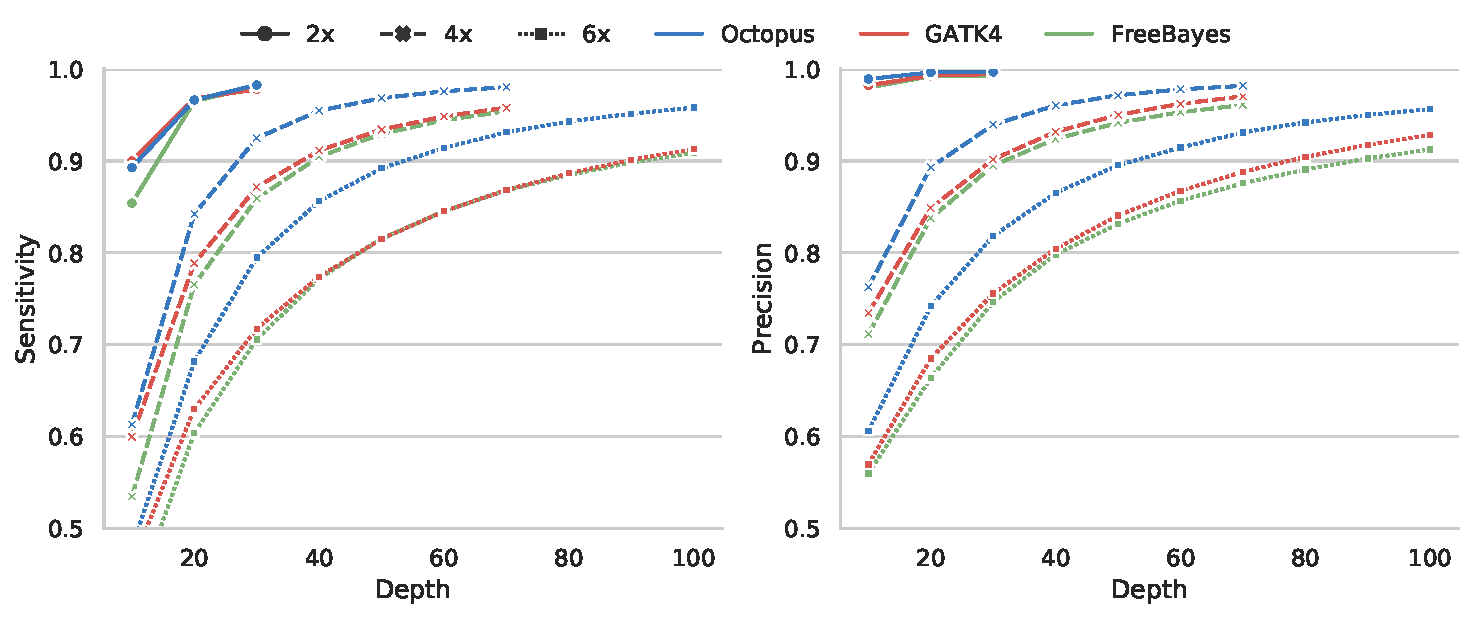
\includegraphics[width=\textwidth]{figures/sensitivity-and-precision-by-depth}
        \label{fig:synthetic:accuracy-by-depth}
    \end{subfigure}
    \begin{subfigure}[b]{\textwidth}
        \vspace{-1cm}
        \caption{}
        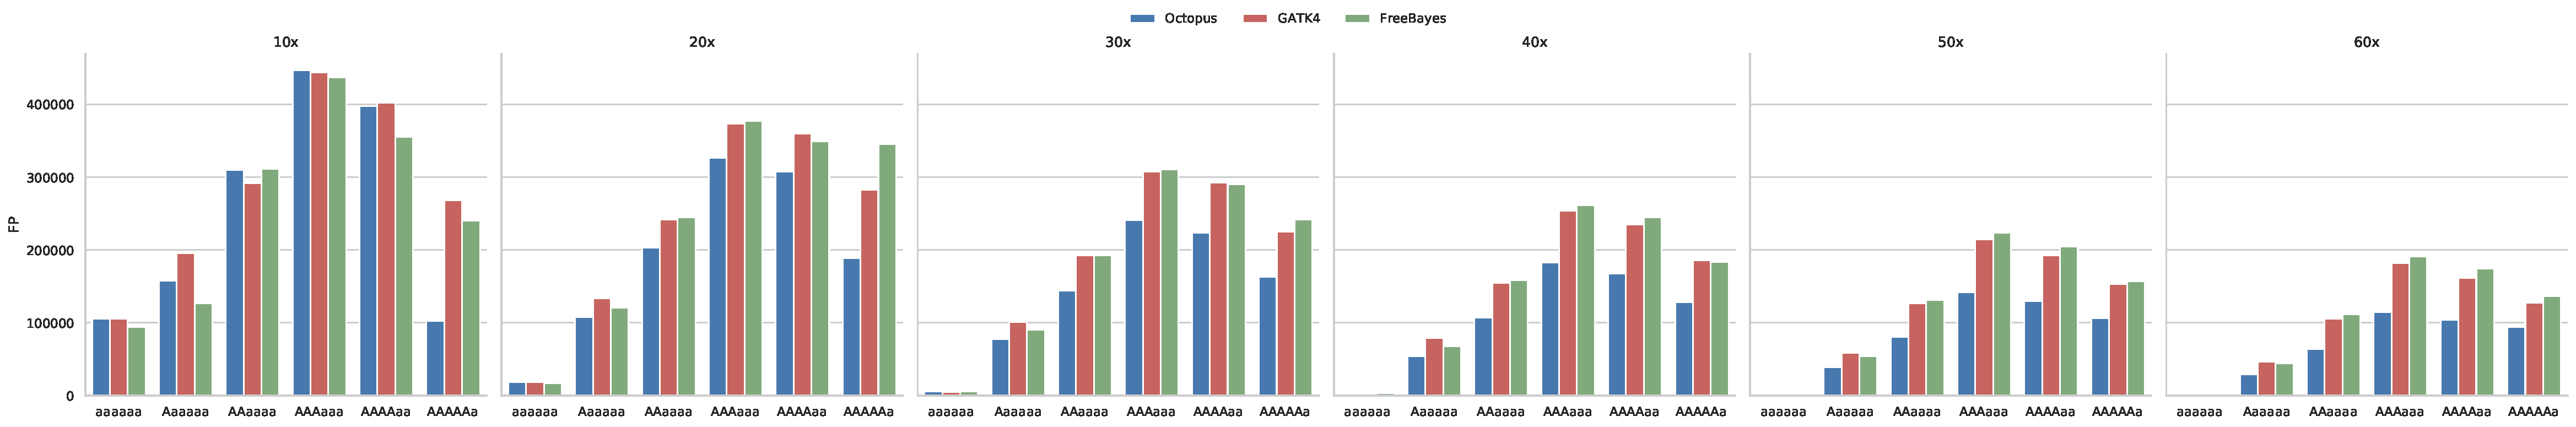
\includegraphics[width=\textwidth]{figures/hexaploid_gt_fp_10-60x}
        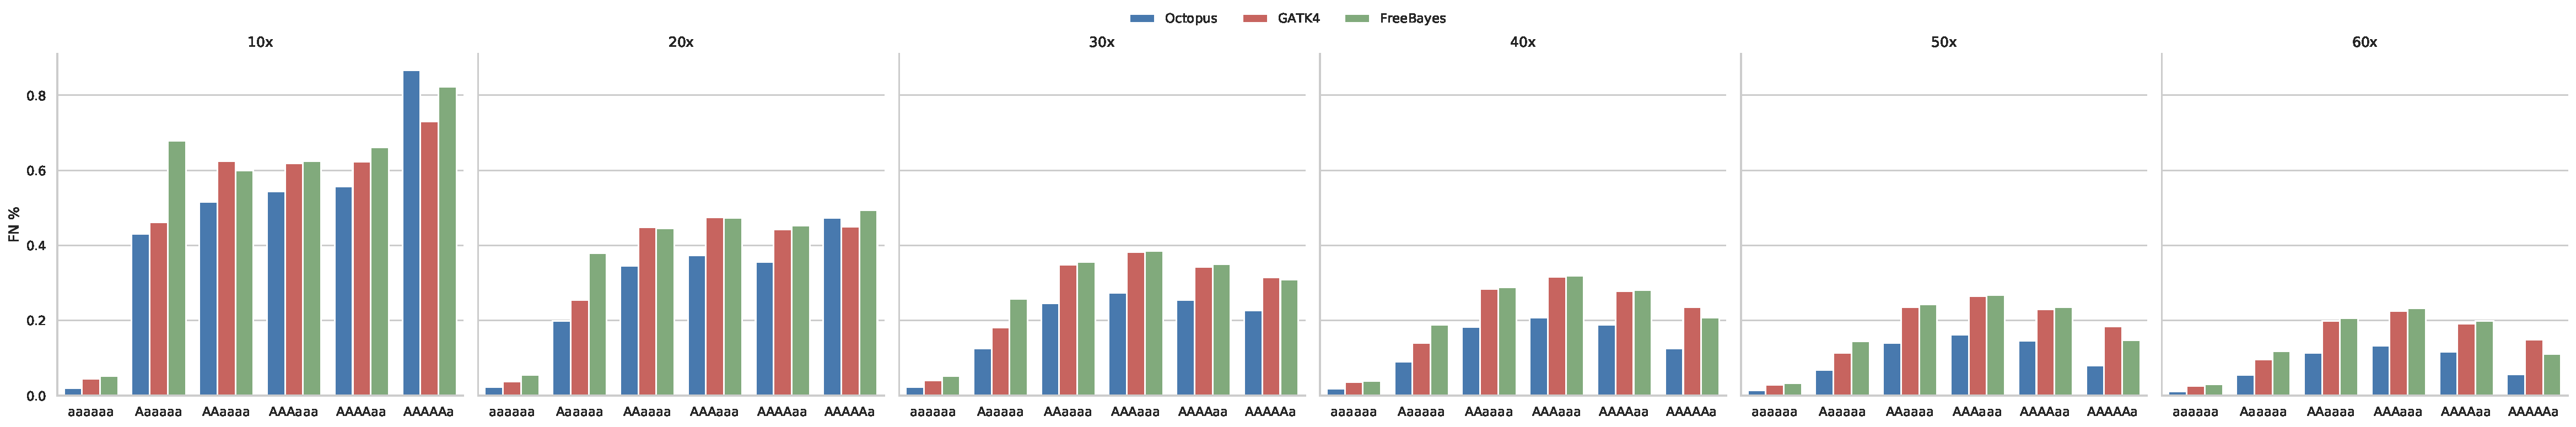
\includegraphics[width=\textwidth]{figures/hexaploid_gt_fn_perc_10-60x}
        \label{fig:synthetic:gt-errors}
    \end{subfigure}
%    \begin{subfigure}[b]{\textwidth}
%     	\vspace{-0.5cm}
%        \caption{}
%        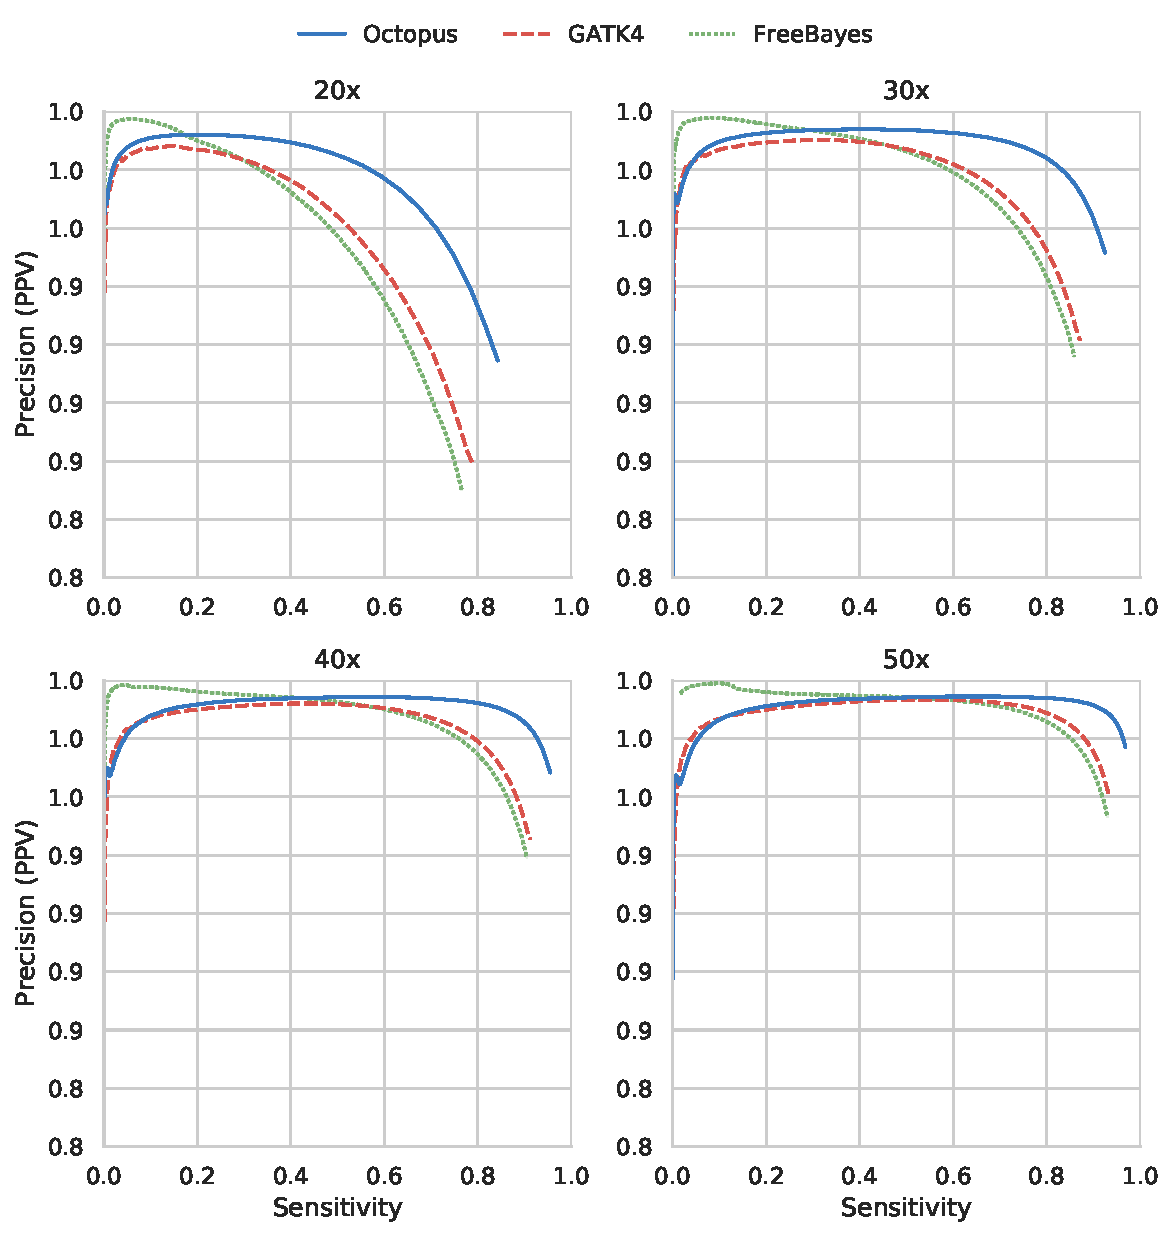
\includegraphics[width=\textwidth]{figures/synthetic-tetraploid-pr-curves_20-50x}
%        \label{fig:synthetic:precision-recall}
%    \end{subfigure}
    \vspace{-0.5cm}
    \caption{\textbf{|\:Genotyping accuracy in synthetic polyploids.} \protect\subref{fig:synthetic:accuracy-by-depth} Sensitivity and precision by depth for each caller on real diploid (2x), and synthetic tetraploid (4x) and hexaploid (6x) Illumina datasets. \protect\subref{fig:synthetic:gt-errors} Counts of false positive biallelic genotypes stratified by depth and copy-number (top). Proportion of false negative biallelic genotypes stratified by depth and copy-number (bottom).}
    \label{fig:synthetic}
\end{figure*}

We evaluated three popular germline variant callers that support polyploid genotypes: Octopus \cite{RN663}; GATK4 \cite{RN598}; and FreeBayes \cite{RN538}, on all synthetic polyploid Illumina datasets, and in the diploid HG002 sample to get performance baselines. Other notable germline callers, such as DeepVariant \cite{RN619}, Strelka2 \cite{RN604}, and Platypus \cite{RN5}, were not included because they do not support polyploid calling. We also ignored methods that  call polyploid SNVs but not indels, such as polyRAD \cite{RN662}. Other than specifying the ploidy, we used nearly default setting for all callers (Supplementary Note $3$). Octopus calls were random forest filtered, GATK4 and FreeBayes calls were hard-filtered using recommended thresholds (Supplementary Note $3$). Variants were compared using RTG Tools \cite{RN169} vcfeval (Supplementary Note $4$).

Genotyping accuracy was considerably lower for polyploids than for diploids. For $30$x sequencing depth, on average $1/200$ diploid genotype calls were incorrect, compared with $1/11$ for tetraploid, and $1/6$ for hexaploid. Sensitivity was similarly affected; there were $8$x and $16$x more false negatives on average for tetraploid and hexaploid, respectively, compared with diploid, for $30$x sequencing. There were also more substantial differences in accuracy between callers for polyploids compared with diploids. Notably, Octopus made on average half the total errors of GATK4 and FreeBayes. There were similar differences for unfiltered calls (Supp Fig $x$). Sequencing depth showed a typical logarithmic relationship with accuracy (F-measure) for both tetraploid and hexaploid samples. The largest F-measure difference between callers occurred at moderate sequencing depth: $30$x for tetraploid, $50x$ for hexaploid. The F-measure also showed a non-linear relationship with ploidy; the performance lost from doubling the ploidy was not recovered by doubling the depth, and the difference increased with depth.

The majority of false positives resulted from incorrect genotype copy-numbers: $x\%$ of false positive biallelic genotype calls ($x\%$ of all false positives) were due to incorrect copy number, although there were notable differences between callers (Fig $x$). The most common false positive for all depths was the balanced heterozygote: AAaa or AAAaaa (Fig. \ref{fig:synthetic:gt-errors}}), of which $x\%$ were due to incorrect copy number. There was no clear bias in the directionality of copy number errors (Supp Fig $x$). The most common biallelic false negatives in tetraploids were heterozygotes with a single variant copy, while for hexaploids it was heterozygotes with two variant copies (Fig. \ref{fig:synthetic:errors1}). However, normalising by the truth prevalence shows that the most frequent false negative for depths $\ge 30$x is the balanced heterozygote for all plodies; for depths $\le 20$x the most frequent false negative was the singleton heterozygote.

Genotype quality scores were well calibrated for all callers, although there was a clear advantage to Octopus' machine learning filtering approach (Fig. \ref{fig:synthetic:precision-recall}); Octopus was the only method where filtering improved F-measure on all tests. 

%\subsection*{Polyploid genotyping accuracy from long-read WGS}


\subsection*{Genotyping in real polyploids}

\begin{figure*}[tp]
	\centering
    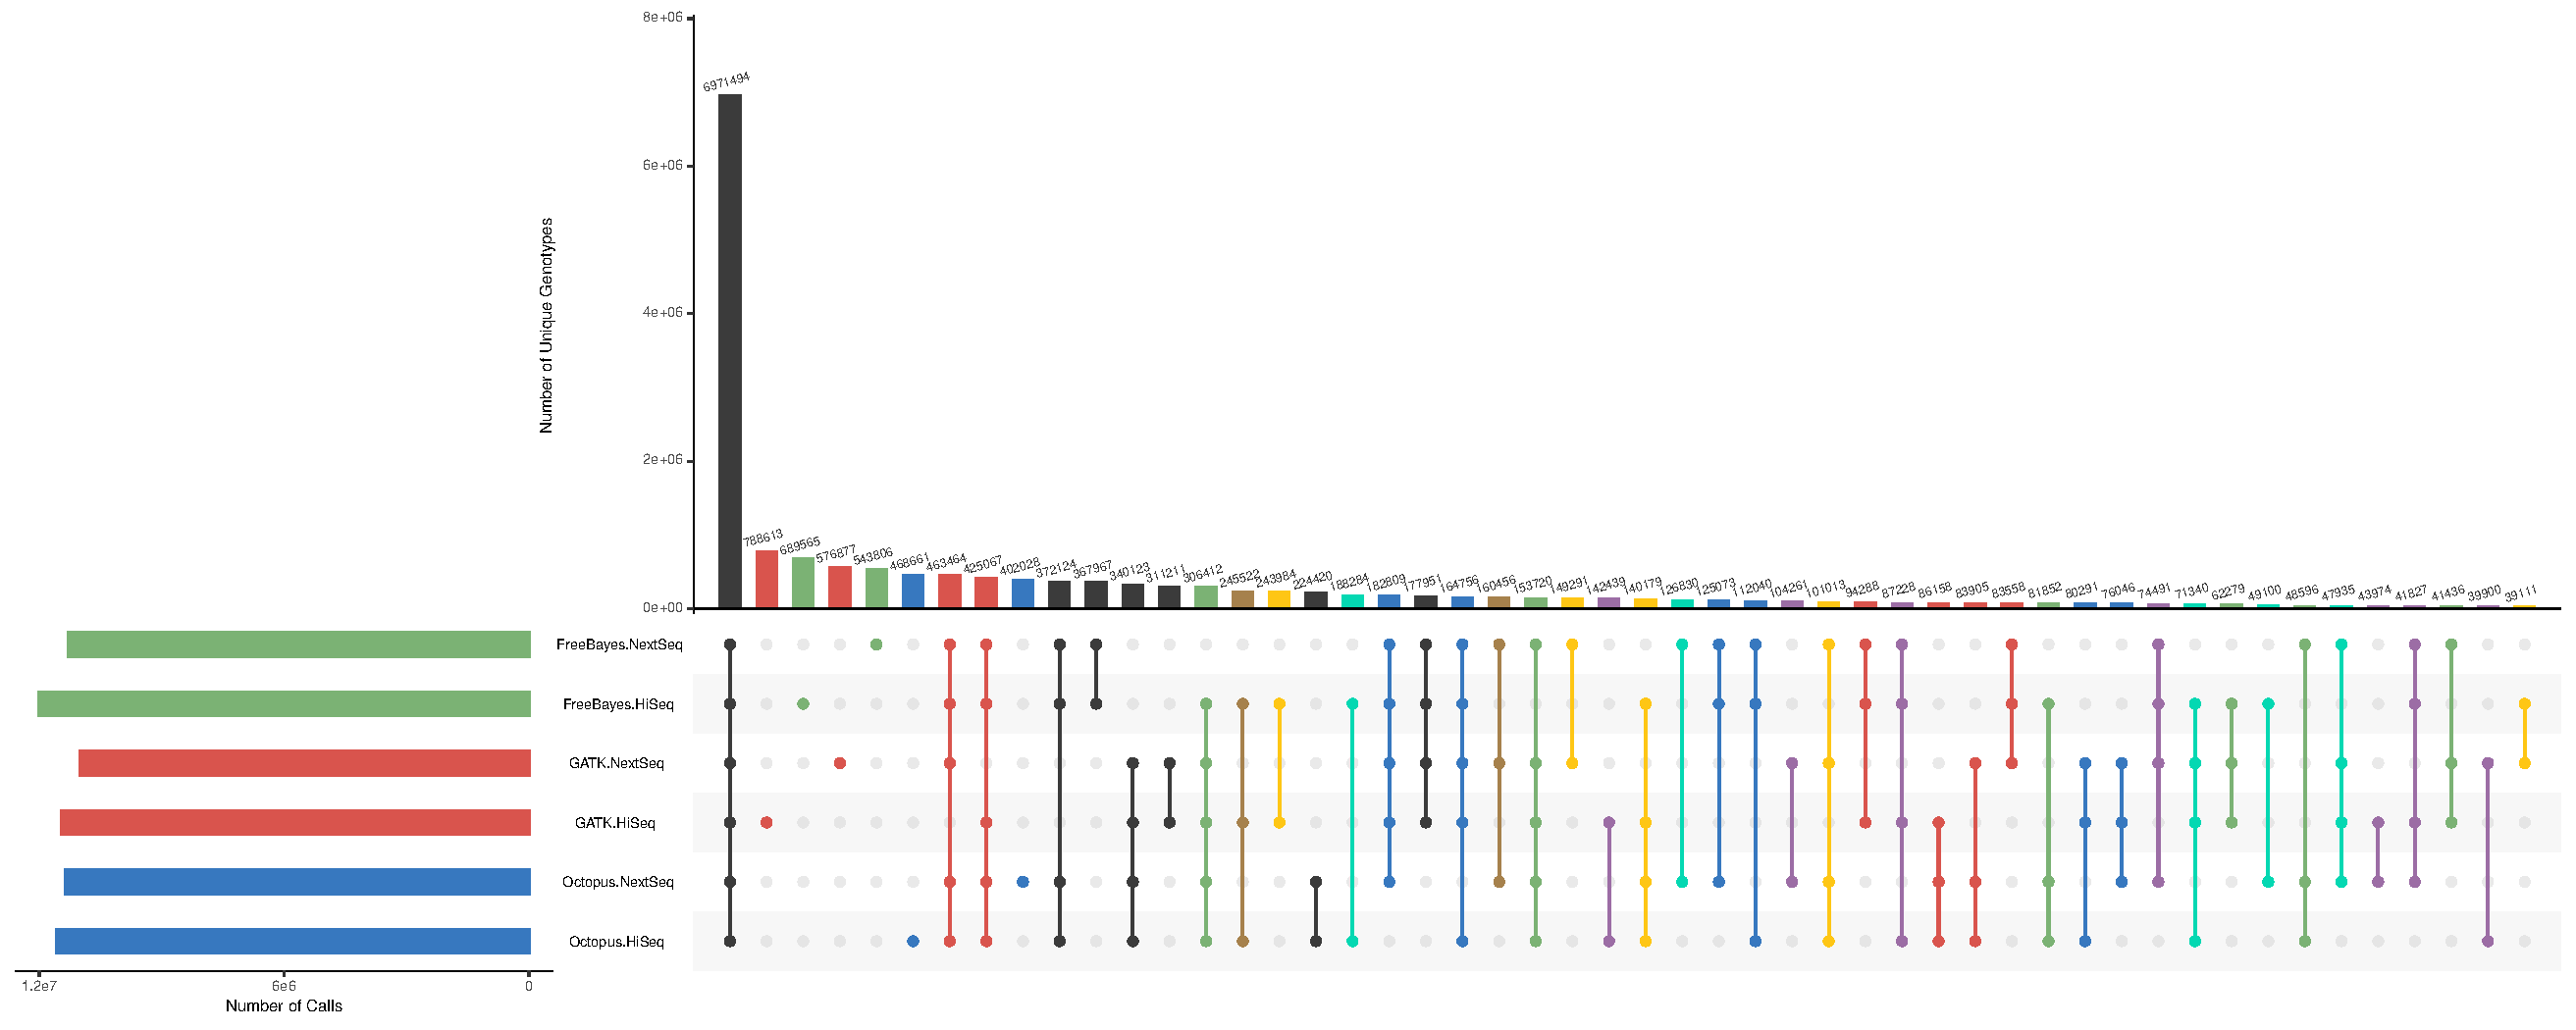
\includegraphics[width=\textwidth,height=0.4\textwidth]{figures/banana_intersection}
    \caption{\textbf{|\:Comparison of genotypes called in two Illumina datasets (HiSeq and NextSeq) of banana specimen by Octopus, GATK4, and FreeBayes}. 'UpSet' plot shows callset intersections for each caller-dataset pair. The largest $50/63$ intersection sets are shown. Intersections are color coded by caller discordance between the two datasets: No discordances (black), Octopus (blue), GATK4 (red), FreeBayes (green), Octopus \& GATK4 (purple), Octopus \& FreeBayes (cyan), GATK4 \& FreeBayes (yellow), All (brown). The total number of unique genotype calls was \num[group-separator={,}]{17277217}.}
    \label{fig:banana_intersection}
\end{figure*}

To support our previous results on real polyploid samples, we called genotypes in recently sequenced banana \cite{RN670} and potato \cite{RN673} specimens. Dwarf Cavendish banana (Musa acuminata) is autotriploid consisting of $11$ chromosomes with a haploid genome size of around $523$Mb, and is an important export-product for many developing countries \cite{RN671}. Potato (Solanum tuberosum) is autotetraploid consisting of $12$ chromosomes with haploid genome size of around $844$Mb \cite{RN668}, and is a vital food source for a large fraction of the world population and is the most cultivated non-grain crop \cite{RN668}. The banana was whole-genome sequenced twice on different machines: once on an Illumina NextSeq-500 to $65$x coverage and once on an Illumina HiSeq-1500 to $55$x coverage. Both datasets were mapped to the DH Pahang v2 reference \cite{RN670}. The potato was whole-genome sequenced on an Illumina to $40$x coverage, and we mapped reads to the Solanum tuberosum DM1-3 reference genome \cite{RN672}. Due to lack of truth data for these samples, we relied on less rigorous means to access the quality of the callsets.

We evaluated the concordance of callers on the two banana datasets with haplotype-aware intersections (Online Methods). The genotype set called by all callers in both datasets, while substantially the largest, only accounted for $40\%$ of all unique genotype calls; $20\%$ of calls were unique to a single callset (Fig. \ref{fig:banana_intersection}). There were also considerable differences between callers: GATK4 had $37\%$ more discordant calls compared with Octopus and $16\%$ more than FreeBayes, despite making less calls overall than FreeBayes and only $3\%$ more than Octopus (Table \ref{table:banana_isec}). We found only slightly higher concordance levels when considering allele matching (Supplementary Fig. $x$ and Supplementary Table $x$); $55\%$ of unique alleles were present in all callsets while $12\%$ were unique to a single callset. Since discordant calls imply at least one false positive or false negative, these results suggests that, unlike for our synthetic data, the majority of false calls arise from unique variant allele calls rather than copy-number errors.

Manual review of discordant calls suggested that a large proportion were due to slightly different proximal indels called in each dataset, suggesting failure to discover correct alleles. To test this, we recalled both datasets with Octopus, using variants called in both datasets by Octopus and GATK4 previously as candidates (Online Methods). The number of called variants increased by $x\%$ and the fraction of concordant calls increased to $x\%$, supporting our hypothesis. Further assessment of a selection of remaining discordant calls using haplotagged and realigned evidence BAMs generated by Octopus indicated that major sources of error were: i) Lack of read depth or allele bias; ii) Missmapped reads, possibly due to incomplete or divergent reference; iii) failure to discover a correct allele (in any callset); iv) Probable structural variation. 



\begin{table}[tp]
\fboxsep0pt %%
\fcolorbox{khaki!20}{khaki!20}{%
\parbox{\linewidth}{%
\fboxsep5pt% 
\caption{\textbf{|\:Concordance in two banana Illumina datasets}}
\label{table:banana_isec}
\vspace{-0.2cm}
\resizebox{\linewidth}{!}   \\
\cmidrule(l{2pt}r{2pt}){1-5}
FreeBayes &  \num[group-separator={,}]{9778611} & \num[group-separator={,}]{3729699} & \num[group-separator={,}]{13508310} & 72\% \\
GATK4     &  \num[group-separator={,}]{9025920} & \num[group-separator={,}]{4421440} &  \num[group-separator={,}]{13447360} & 67\% \\
Octopus   &   \num[group-separator={,}]{9854737} & \num[group-separator={,}]{3219611} & \num[group-separator={,}]{13074348} & 75\% \\
\end{tabular}%
}%
}%
}%
\end{table}

\section*{Discussion}

We have shown that polyploids can be reliably variant called for moderate sequencing depths (e.g. $\ge30$x), but accurate genotyping remains challenging for sequencing depths below $60$x. We showed that there is considerably less concordance between variant calling methods for polyploids than diploids, and that Octopus substantially outperforms other methods, including GATK4 and FreeBayes, particularly for genotyping.

Our analysis is not without limitations. Our most reliable analysis was on human genomic data, but most polyploid genomes are more challenging to call than human genomes due to higher repetitiveness, less complete references, and higher reference divergence. These challenges likely explain why the upper-bounds on precision that we calculated from the banana datasets were considerably lower than would be expected via extrapolation from our synthetic tetraploid tests. Notably, the divergence of the banana sample from the reference was substantially higher than the human sample. Moreover, our study focuses on small variants, but polyploids, including many plants, are highly susceptible to structural changes, including copy-number changes. Furthermore, without a  ground truth it is very difficult to have high confidence in sensitivity. We therefore stress the importance of treating our performance figures on synthetic polyploid data as upper bounds of what can be achieved when applying the same methods to real polyploid data.

We have only considered single sample polyploid calling in this work, however, multi-sample calling is  important for studying population diversity. Population calling in humans is a difficult problem due to the computational complexities of joint calling and difficulties in merging independent callsets. Population calling in polyploids will likely be even more challenging, and would perhaps benefit from  more sophisticated genotype priors as developed in other methods \cite{RN666}.

In summary, we have conducted the most comprehensive study on genotyping errors in polyploids to date. We found considerable differences in performance between variant calling methods, but 

\bibliographystyle{naturemag}
\bibliography{references}

\section*{Online methods}\small

\paragraph*{Code availability.} Octopus source code and documentation is freely available under the MIT licence from \url{https://github.com/luntergroup/octopus}. Custom Python code used for data analysis is available from \url{https://github.com/luntergroup/polyploid}.

\paragraph*{Data availability.} All primary data used for analysis is available from public sources. Links are provided in Supplementary Note $x$ and can also be found, along with automatic download options, in the online code (\url{https://github.com/luntergroup/polyploid}). Synthetic data can easily be reproduced using the online code.

\paragraph*{Acknowledgements.} We would like to thank Len Trigg at Real Time Genomics for kindly updating RTG Tools to support polyploid genotypes. The computational aspects of this research were supported by the Wellcome Trust Core Award Grant Number 203141/Z/16/Z and the NIHR Oxford BRC. The views expressed are those of the author(s) and not necessarily those of the NHS, the NIHR or the Department of Health.

\paragraph*{Author contributions.} D.P.C did the analysis and wrote the paper. D.W. and G.L critically reviewed the manuscript and supervised the project.

\end{document}